 \chapter{DYNAP-SE1 Visualization and interactive control tools}
 \label{appendix:dynapse_gui}

 \section{Bias Slider GUI}

 A class providing a visual interface for control over every bias of every core for the case when the Samna instance with a DYNAP-SE1 board is running locally. The requirements for the GUI to work correctly are the packages \pyobject{samna}, \pyobject{matplotlib} and \pyobject{tkinter}.
\\
The interactive GUI module only functions for the DYNAP-SE1 boards connected locally.
\\
\noindent The code is available within the DYNAP-SE1 software repository in the \verb|live_gui| subfolder:\\

\textbf{Link:} \url{https://code.ini.uzh.ch/ncs/libs/dynap-se1/-/tree/main/live_gui}

\bigskip
\noindent\textbf{Initialization}\\

To initialize the GUI, a function \verb|run_threaded_gui| needs to be imported from the \pyobject{SliderGui} class so that it runs in a separate process and does not block the active Python interpreter. After opening the DYNAP-SE1 board, pass the object \verb|model| returned by the \verb|ut.open_dynapse1()| function to that Slider Gui thread spawning function.

\begin{lstlisting}[language=Python, caption=Slider Gui initialization]
import samna
import dynapse1utils as ut

from live_gui.sliderGui import run_threaded_gui

model, gui_thread = ut.open_dynapse1(gui=True)

run_threaded_gui(model)

\end{lstlisting}

A window will appear (see example in Figure ~\ref{fig:bias_gui_screenshot}, containing interactive sliders for all biases of each core of the board. The bias pages are organized as one column per core, with four tabs one for each chip. Each bias is labelled as they are named on the chip layout, but below you can find a brief explanation for most of them.

\begin{figure}[h!]
    \centering
        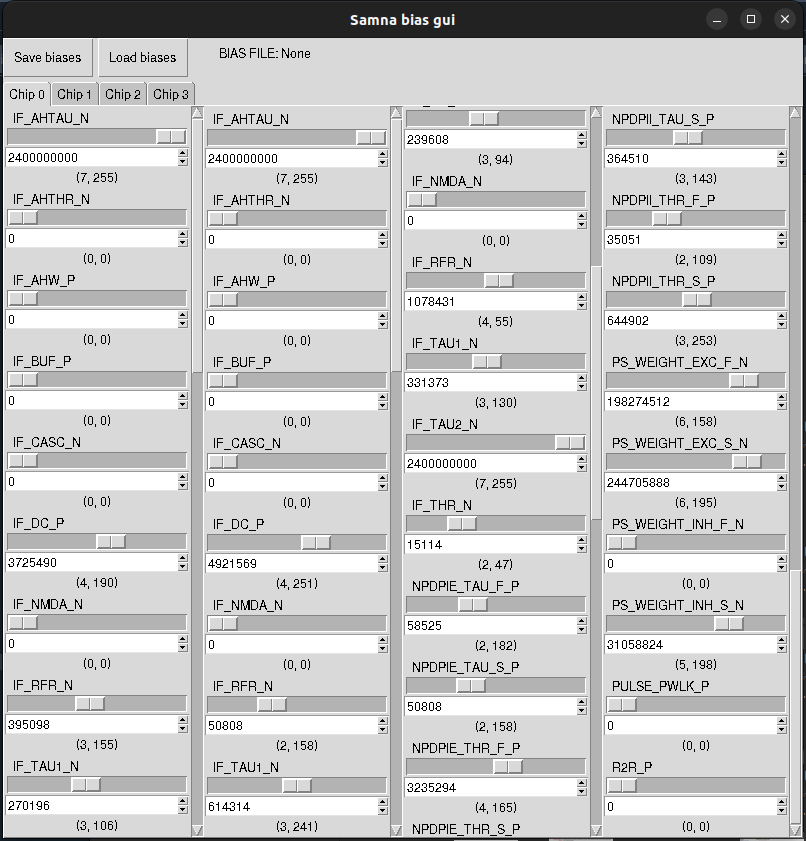
\includegraphics[width=0.9\textwidth]{img/appendices/Bias_gui_screenshot.png}
    \caption[Bias GUI screenshot]{Graphical user interface for the DYNAP-SE1 bias control with Samna.}
    \label{fig:bias_gui_screenshot}
\end{figure}

The biases are set in their \emph{linear} values, meaning the range from the minimum to the maximum values is covered by one continuous variable. The value of that linear bias is visible in the corresponding spin boxes and can by typed in for precision. The on-chip bias generators accept the \emph{coarse} and \emph{fine} values, but the conversion is done using the lookup table:

\begin{table}[h!]
\begin{tabularx}{\textwidth}{|c|X|}
\hline
\textbf{Bias name}   & \textbf{Property} \\
\hline
\multicolumn{2}{c}{Adaptive firing threshold block} \\
\hline
\verb|IF_AHTAU_N| & Neuron firing frequency adaptation time constant\\ 
\verb|IF_AHTHR_N| & DPI threshold for the adaptation (max value)\\ 
\verb|IF_AHW_P| & Neuron time constant \\ 
\verb|IF_CASC_N| & Enables firing threshold adaptation \\ 
\hline
\multicolumn{2}{c}{Neuron parameters} \\
\hline
\verb|IF_DC_P| & DC current injected into a neuron \\ 
\verb|IF_NMDA_N| & Enable NMDA gating \\ 
\verb|IF_RFR_N| & Neuron refractory period \\ 
\verb|IF_TAU1_N| & Neuron time constant \\ 
\verb|IF_TAU2_N| & Secondary neuron time constant; can be selected through API with the \verb|set_to_tau2()| function\\ 
\verb|IF_THR_N| & Neuron \verb|V_mem| gain (not the firing threshold!) \\ 
\hline
\multicolumn{2}{c}{Synapse parameters} \\
\hline
\verb|NPDPIE_TAU_F_P| & Fast excitatory (\verb|AMPA|) synapses time constant\\ 
\verb|NPDPIE_TAU_S_P| & Slow excitatory (\verb|NMDA|) synapses time constant\\ 
\verb|NPDPIE_THR_F_P| & Fast excitatory (\verb|AMPA|) synapses DPI threshold (i.e. max synaptic current value)\\ 
\verb|NPDPIE_THR_S_P| & Slow excitatory (\verb|NMDA|) synapses threshold (i.e. max synaptic current value)\\ 
\verb|NPDPII_TAU_F_P| & Fast inhibitory (\verb|GABA_A|) synapses time constant\\ 
\verb|NPDPII_TAU_S_P| & Slow inhibitory (\verb|GABA_B|) synapses time constant\\ 
\verb|NPDPII_THR_F_P| & Fast inhibitory (\verb|GABA_A|) synapses threshold\\ 
\verb|NPDPII_THR_S_P| & Slow inhibitory (\verb|GABA_B|) synapses threshold\\ 
\verb|PS_WEIGHT_EXC_F_N| & Fast excitatory (AMPA) synapse weights\\ 
\verb|PS_WEIGHT_EXC_S_N| & Slow excitatory (NMDA) synapse weights\\ 
\verb|PS_WEIGHT_INH_F_N| & Fast inhibitory (\verb|GABA_A|) synapse weights\\ 
\verb|PS_WEIGHT_INH_S_N| & Slow inhibitory (\verb|GABA_B|) synapse weights\\ 
\hline
\multicolumn{2}{c}{Auxiliary} \\
\hline
\verb|PULSE_PWLK_P| & Pulse width for synapse circuits\\ 
\hline
\end{tabularx}
\label{tab:bias_names_list}
\caption{List of biases available to control on DYNAP-SE1 and their meaning}
\end{table}



\bigskip
\noindent\textbf{Loading and saving the biases}
\bigskip

Above the bias blocks, two buttons allow to load and save the current state of the bias configuration from and to the location of choice.

Any interaction with the GUI instantly applies the changes to the DYNAP-SE1 board, meaning the user can move the slider and observe the effect of the changed parameter live on the \pyobject{Samna}'s spike monitor or in the change of the analog voltage trace on the attached oscilloscope.

At the same time, if some of the biases are changed from the code in the main Python process or any other script, the changes will be reflected in the GUI, as it refreshes the state of the \pyobject{model} object with a fixed rate.



%\newpage
%\section{WTA online plotting}